\newpage
\selectlanguage{ukrainian}
\section{Стаціонарне рівняння та його розв'язки}
\subsection{Перехід до стаціонарного рівняння та метод його розв'язку}
\hspace*{8mm} Для дослідження динаміки пучків потрібно вирішити який сигнал подавати на вхід. Доцільно було б подати на вхід розв'язок якогось стаціонарного рівняння.

Нехай $\Psi_n(x,y,z)=\psi_n(r)e^{i\Lambda_n z+im_n\varphi},$, а потім зробивши рескалювання $\psi_n\to\psi_n/\alpha$, $\theta\to\theta/\alpha^2$ отримаємо
\begin{equation}
   \begin{array}{l} {\displaystyle
       -\lambda_n \psi_n(r)+\Delta_r^{(m_n)}\psi_n(r) +\theta\psi_n(r)=0,
       } \\*[9pt] {\displaystyle
\,\,\theta-\Delta_r^{(0)}\theta=|\psi_1|^2+|\psi_2|^2,
   }\end{array}
   \label{eq:StatNLS}
\end{equation}
де  $\lambda_n=\Lambda_n/\alpha^2$,
$\Delta_r^{(m)}=\frac{d^2}{dr^2}+\frac{1}{r}\frac{d}{dr}-\frac{m^2}{r^2}$.
Граничні умови: $\psi_n(0)=0$ якщо $m\ne0$ та $\psi'_n(0)=0$, якщо $m=0$; $\psi(+\infty)=0$. Зазначимо, що в нелокальному ліміті $\alpha^2\ll 1$ еквівалентно великим значенням $\lambda_n$. Таким чином, в перенормованих змінних $\lambda_n$ є мірою нелокальності середовища.

Розрахунок проводиться методом релаксації та стабілізації. Перепишемо наші рівняння у вигляді:
\begin{equation}
   \begin{array}{l} {\displaystyle
       \lambda_n \psi_n(r)-\Delta_r^{(m_n)}\psi_n(r)=\theta\psi_n(r),
       } \\*[9pt] {\displaystyle
\,\,\theta-\Delta_r^{(0)}\theta=|\psi_1|^2+|\psi_2|^2.
   }\end{array}
   \label{eq:StatNLS1}
\end{equation}

Позначимо оператор $\hat{L_m}=\lambda_n-\Delta_r^{(m_n)}$, тоді

\begin{equation}
   \begin{array}{l} {\displaystyle
       \hat{L_m} \psi_n(r)=\theta\psi_n(r),
       } \\*[10pt] {\displaystyle
\,\theta-\Delta_r^{(0)}\theta=|\psi_1|^2+|\psi_2|^2.
   }\end{array}
   \label{eq:StatNLS2}
\end{equation}

Суть методу в тому, що ми вибираємо початкову функцію $\psi_n^{(0)}$, потім розраховуємо $\theta^{(0)}$ з

\begin{equation}
\theta^{(0)}-\Delta_r^{(0)}\theta^{(0)}=|\psi_1^{(0)}|^2+|\psi_2^{(0)}|^2.
\end{equation}

Наступним кроком є розрахунок $\psi_n^{(0)}$ з
\begin{equation}
\hat{L_m} \psi_n^{(1)}(r)=\theta^{(0)}\psi_n^{(0)}(r),
\end{equation}

після чого, ми робимо стабілізацію розв'язку:
\begin{equation}
\psi_n^{(1)}(r) = (S_n^{(0)})^{0.7} \psi_n^{(1)}(r),
\end{equation}

де $S$ - стабілізаційний коефіцієнт:
\begin{equation}
S_n^{(0)} = \dfrac{\int_{0}^{\infty}(\psi_n^{(1)})^2 dr}{\int_{0}^{\infty}(\psi_n^{(0)})^2 dr}.
\end{equation}

А далі маємо ітераційний процес:

\begin{equation}
   \begin{array}{1} \displaystyle
           \theta^{(i+1)}=(1-\Delta_r^{(0)})^{-1}(|\psi_1^{(i)}|^2+|\psi_2^{(i)}|^2),
           \\*[10pt]
          \displaystyle
                  \psi_n^{(i+1)}(r)=\hat{L_m}^{-1}(\theta^{(i)}\psi_n^{(i)}(r)),
                 \\*[10pt] \displaystyle
\,\,\psi_n^{(i+1)}(r) = (S_n^{(i)})^{0.7} \psi_n^{(i+1)}(r).
  \end{array}
\end{equation}

Початковою пробною функцією виберемо $\psi_n(r)=exp(-r)r^m$, як таку, що задовільняє граничним умовам. 

\subsection{Існування векторних розв'язків}
\hspace*{8mm} Вирішуючи  систему рівнянь (\ref{eq:StatNLS2}) з $m_1=m_2$ та $\lambda_1\ne\lambda_2$, ми отримаємо цікавий результат: одна з компонент зануляється, тобто при різних $\lambda_n$ існують лише скалярні розв'язки.

Щоб проілюструвати це, перейдемо до більш загального вигляду рівняння, з урахуванням кросс-модуляції фази:
\begin{equation}
   \begin{array}{l} {\displaystyle
       \hat{L_m} \psi_n(r)=\theta_n\psi_n(r),
       } \\*[10pt] {\displaystyle
\,\theta_n-\Delta_r^{(0)}\theta_n=\hat\sigma_{ni}|\psi_i|^2,
   }\end{array}
   \label{eq:StatNLScross}
\end{equation}

де
\begin{equation}
\hat\sigma_{ni}=\begin{pmatrix} 1 & \sigma \\ \sigma & 1 \end{pmatrix}.
\end{equation}

При $\sigma=1$ ми отримаємо систему (\ref{eq:StatNLS2}).
Побудуємо діаграму залежностей $N_1(\lambda_1,\lambda_2)$ та $N_2(\lambda_1,\lambda_2)$ для фіксованого значення $\lambda_1+\lambda_2=1$ та $\sigma=0.8$

\begin{figure}[h]
  \centering
  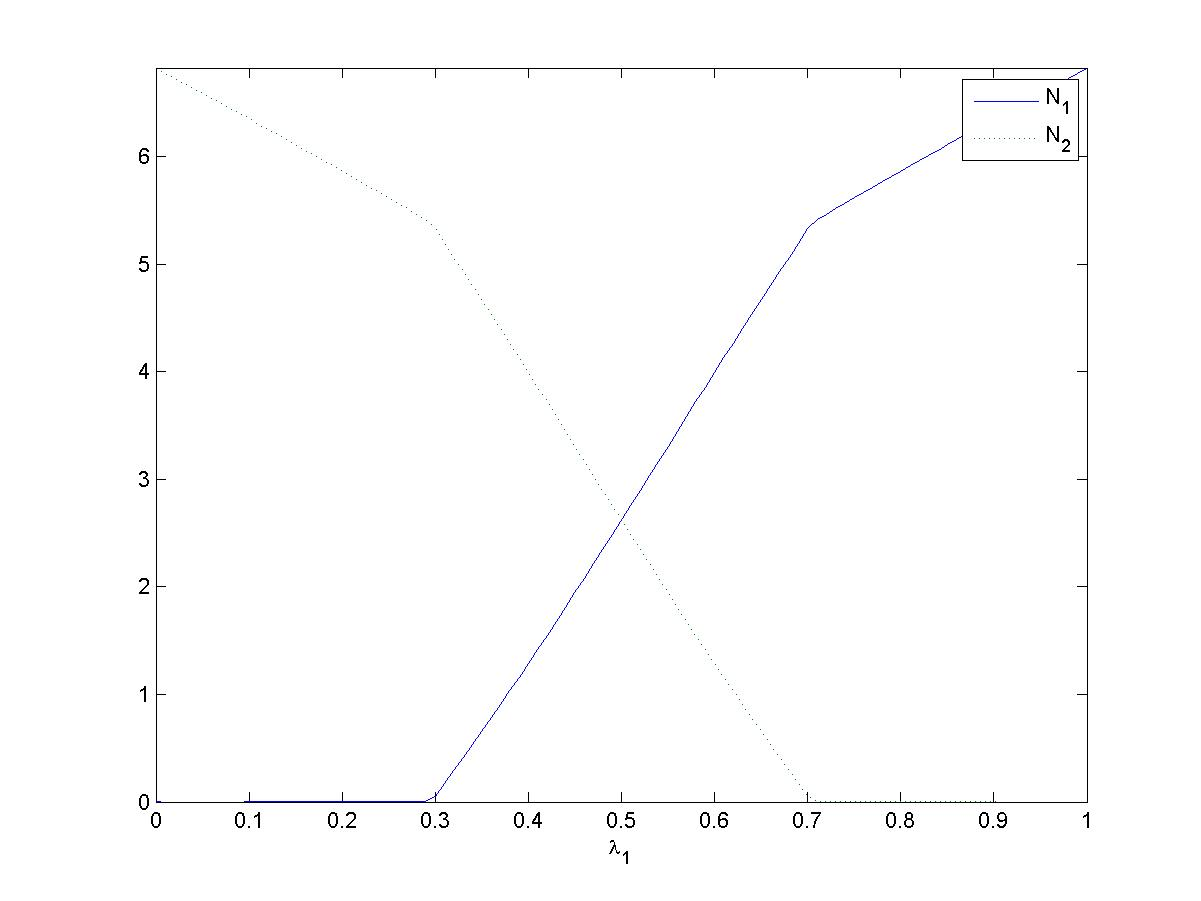
\includegraphics[width=450pt]{fig2}
  \label{fig2}
\end{figure} 

Як бачимо, існує лише невелика область ($0.29<\lambda_1<0.71$) де існують векторні розв'язки.

Чим менше $\sigma$ буде відрізнятися від одиниці, тим менша буде ця область:

\begin{figure}[h]
\begin{minipage}[h]{0.49\linewidth}
\center{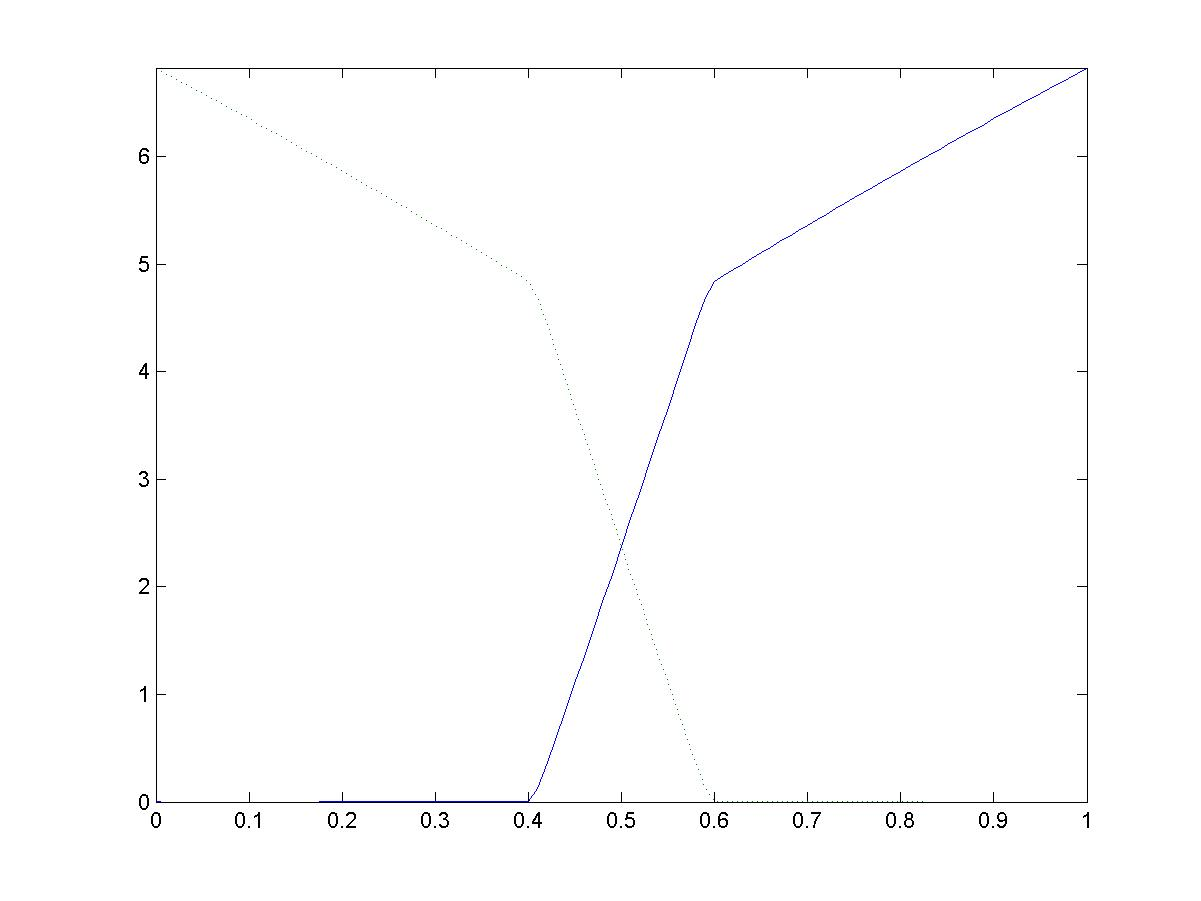
\includegraphics[width=220pt]{fig3_1}} a
\end{minipage}
\hfill
\begin{minipage}[h]{0.49\linewidth}
\center{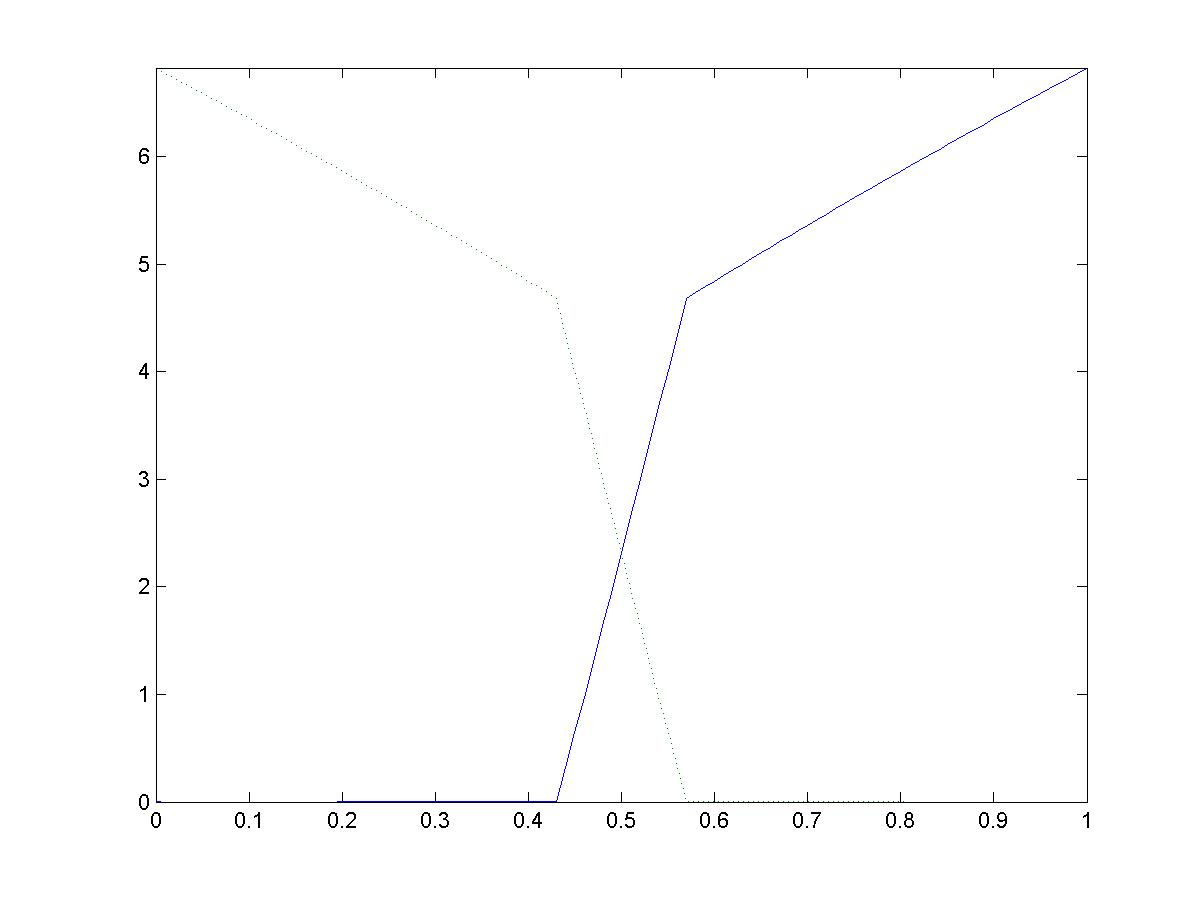
\includegraphics[width=220pt]{fig3_2}} b
\end{minipage}
\vfill
\begin{minipage}[h]{0.49\linewidth}
\center{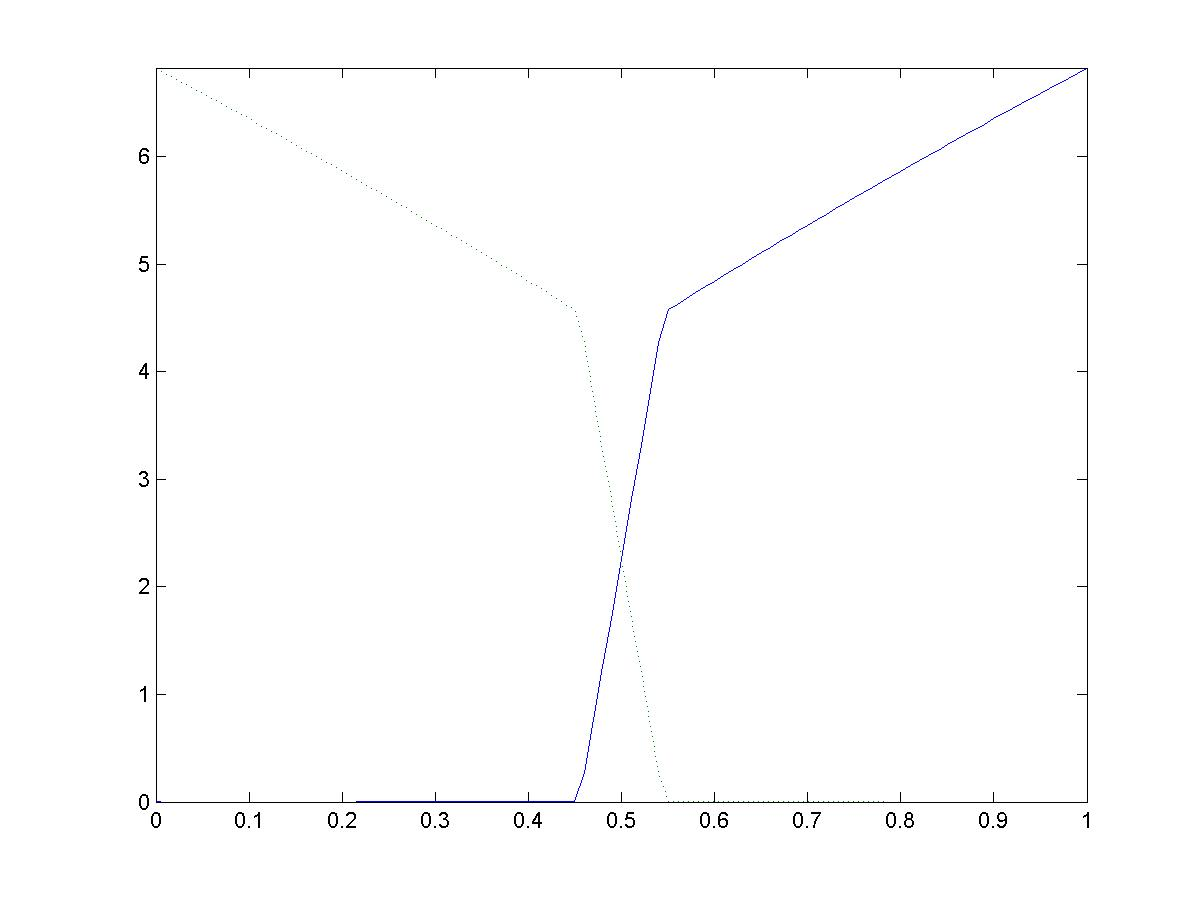
\includegraphics[width=220pt]{fig3_3}} c
\end{minipage}
\hfill
\begin{minipage}[h]{0.49\linewidth}
\center{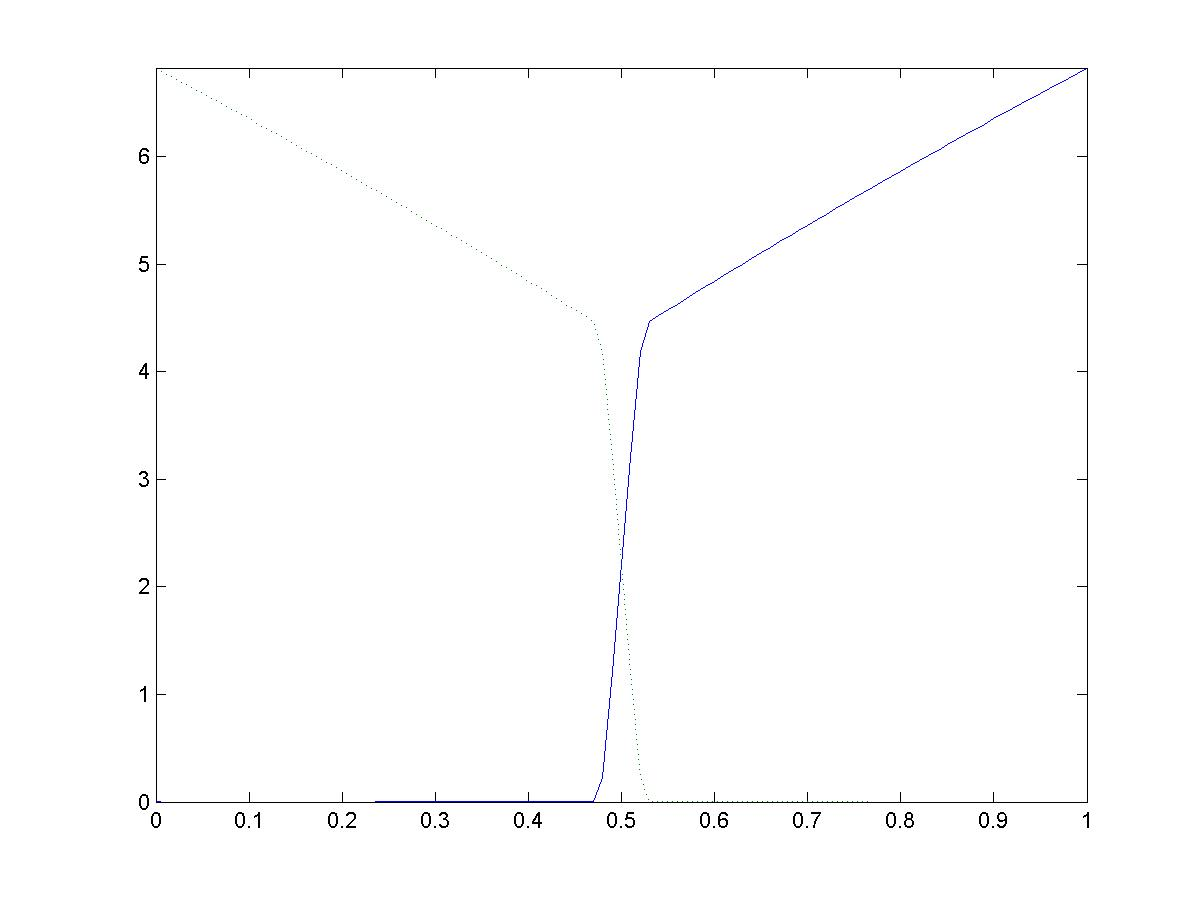
\includegraphics[width=220pt]{fig3_4}} d
\end{minipage}
\caption{Профілі $N_1(\lambda_1,\lambda_2),N_2(\lambda_1,\lambda_2)$ для $a)\, \sigma = 0.9,\, b)\, \sigma = 0.925, \, c)\, \sigma = 0.95,\, d)\, \sigma = 0.975$ }
\end{figure}

Для $\sigma\approx1$ область існування векторних розв'язків буде нульова. 

\subsection{Типові розв'язки стаціонарного рівняння}
\hspace*{8mm} В попередньому параграфі ми отримали цікавий ефект. Однак в системі, що розглядається нами не береться до уваги кросс-модуляція фази, отже векторні розв'язки будуть існувати лише на прямій $\lambda_1=\lambda_2$. Позначимо цю зміннуу $\lambda$, і надалі ми користуватимемося нею та розглядатимемо лише такі вихори.

На малюнках показані чисельно отримані типові профілі $\psi_n(r)$ та $\theta(r)$ для різних $\alpha$ та $\lambda=0.1$:

\begin{figure}[h]
  \centering
  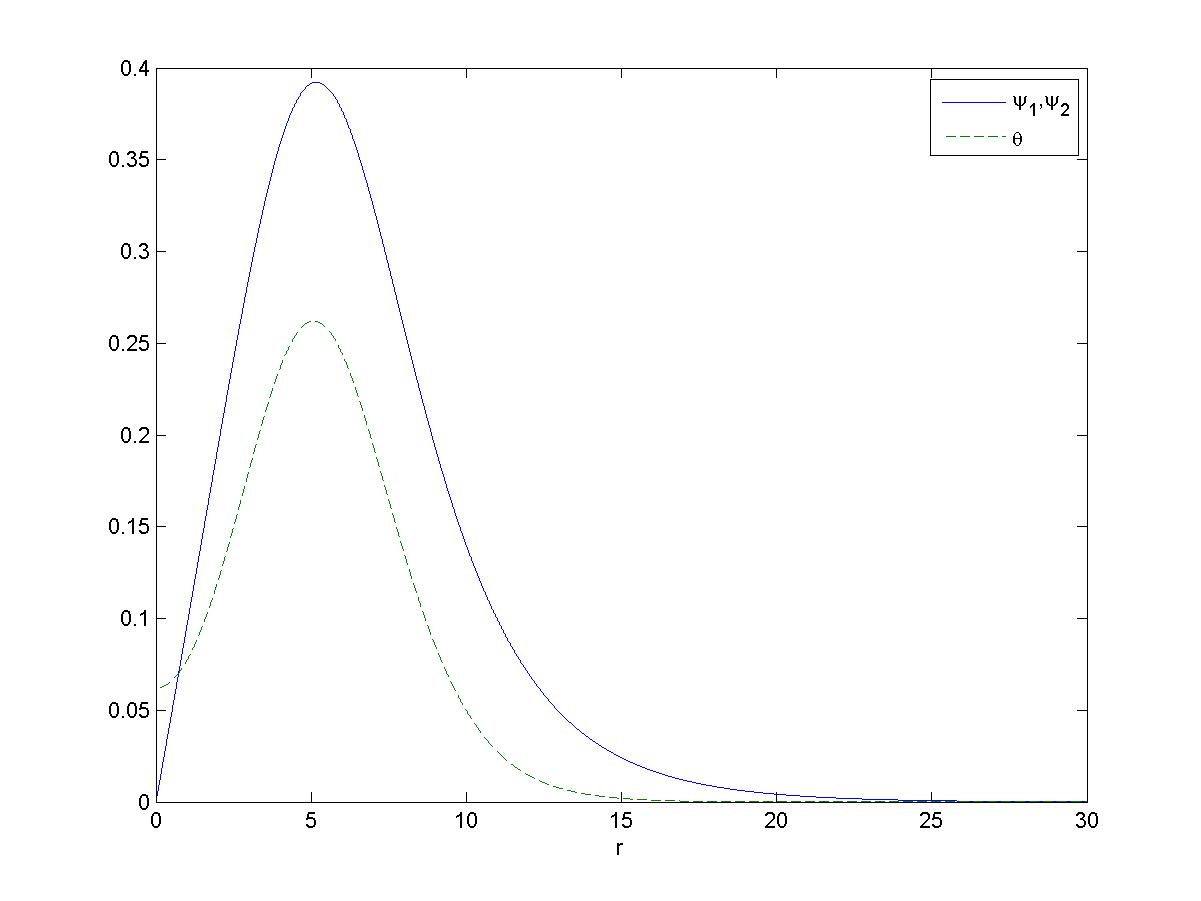
\includegraphics[width=300pt]{fig4_3}
  \caption{$\alpha=1$} 
\end{figure} 
\begin{figure}[h]
  \centering
  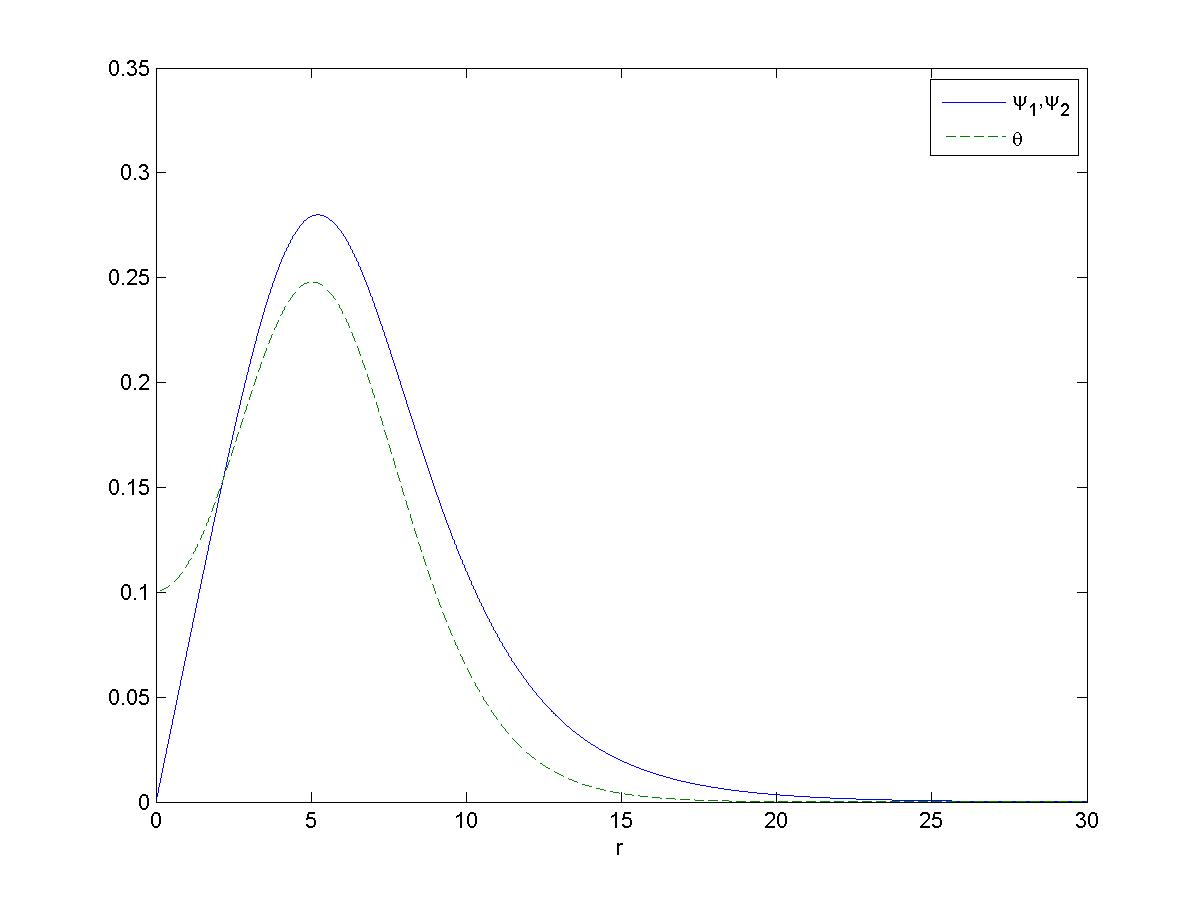
\includegraphics[width=300pt]{fig4_4}
  \caption{$\alpha=0.5$} 
\end{figure} 
\begin{figure}[h]
  \centering
  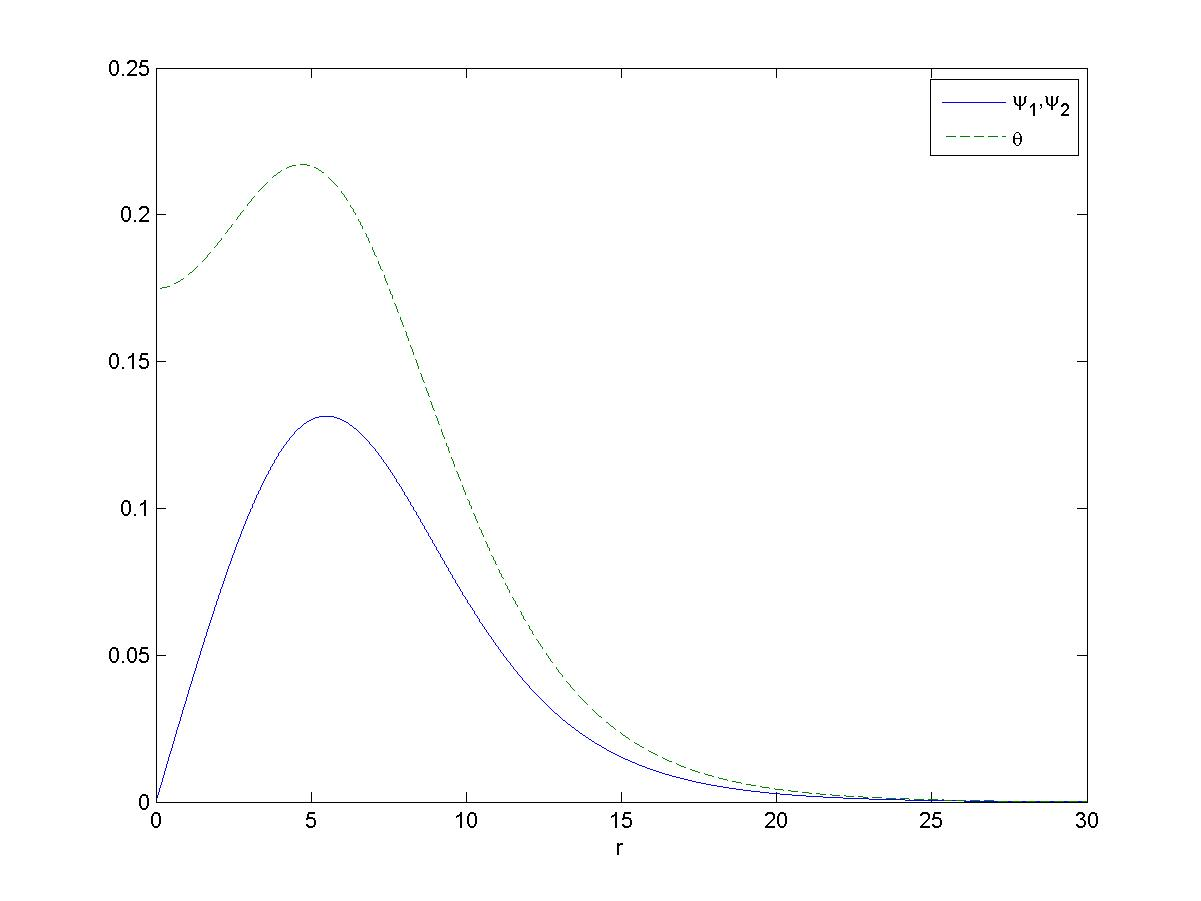
\includegraphics[width=300pt]{fig4_5}
  \caption{$\alpha=0.1$} 
\end{figure} 
